\section{$e^{-}$ vs. $\gamma$ Particle Identification}
Given a reconstructed electromagnetic (EM) shower, a particle type is assigned as $e^{-}$ or $\gamma$ using
a log-likelihood ratio ($\mathcal{LL}$) method. This appendix describes about both a procedure and algorithm source code repository.

\subsection{Procedure}
There are two probability density functions (PDFs) defined and used for likelihood calculation: one
is for a particle's radiation length [cm], and the other for dE/dX [MeV/cm]. The former is a simple
exponential function while the latter is a simple gaussian for electron and double-gaussian for gamma.
A reason for using double-gaussian for gamma's dE/dX is to account for a small peak at 2 MeV/cm for gamma
showers with a mis-reconstructed start point.
\begin{eqnarray}
  \text{Radiation Length PDF}_{e^{-}/\gamma} &=& \exp\left(-x/\mathcal{L}_{rad.}\right)\\
  \text{dE/dx PDF}_{e^{-}} &=& \exp\left(-\frac{(x-\mu)^2}{2\sigma^2}\right)\\
  \text{dE/dx PDF}_{\gamma} &=& \exp\left(-\frac{(x-\mu_1)^2}{2\sigma_1^2}\right) + N\times\exp\left(-\frac{(x-\mu_2)^2}{2\sigma_2^2}\right)
\end{eqnarray}
\begin{figure}[htb]
\begin{center}
  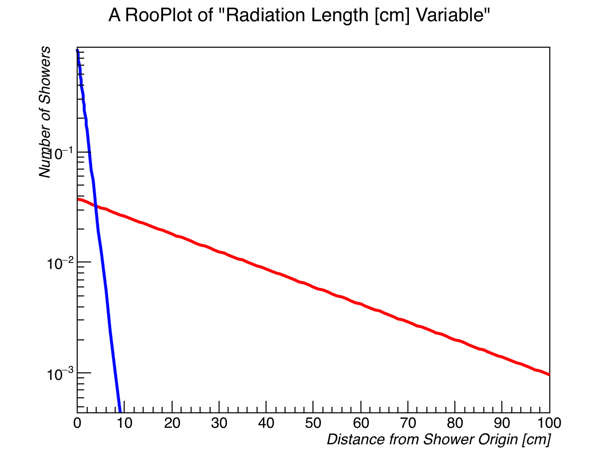
\includegraphics[width=3in]{RadLength.png}
  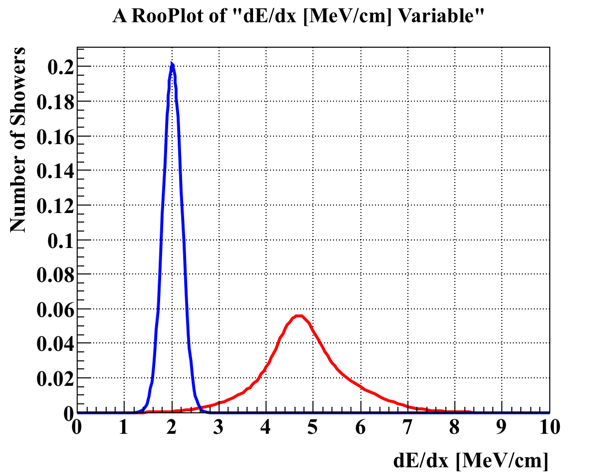
\includegraphics[width=3in]{dEdx.png}
  \caption{Probability density function of a radiation length [cm] (left) and dE/dx [MeV/cm]
    for electron (blue) and gamma ray (red). Values are tuned using MCReco information from single
    $e^{-}$ and $\gamma$ MC samples.}
  \ref{fig:algoempart}
\end{center}
\end{figure}
The default parameter set for these PDFs are tuned using MCReco showers from single $e^{-}$ and $\gamma$
MC sample with an artificially widened width which comes from a resolution from reconstructed shower.
This is shown in Fig.\ref{fig:algoempart}.

Then electron/gamma likelihood is defined as
\begin{eqnarray}
  \mathcal{LL}_{e^-}\left(dE/dx,\mathcal{L}_{rad}\right) &=& \frac{\text{PDF}_{e^-}(dE/dx,\mathcal{L}_{rad})}{\text{PDF}_{e^-}(dE/dx,\mathcal{L}_{rad}) + \text{PDF}_{\gamma}(dE/dx,\mathcal{L}_{rad})}\\
    \mathcal{LL}_{\gamma}\left(dE/dx,\mathcal{L}_{rad}\right) &=& \frac{\text{PDF}_{\gamma}(dE/dx,\mathcal{L}_{rad})}{\text{PDF}_{e^-}(dE/dx,\mathcal{L}_{rad}) + \text{PDF}_{\gamma}(dE/dx,\mathcal{L}_{rad})}
\end{eqnarray}
and a particle type of each EM shower is assigned based on above formula with higher return value.

\subsection{Toolkit}
The procedure described above is implemented in a {\ttfamily C++} toolkit {\ttfamily ERTool}.
In particular {\ttfamily ertool::AlgoEMPart} is responsible for this $e^-$ vs. $\gamma$ separation
method in {\ttfamily ertool::AlgoEMPart::LL} function. One can find a source code at
\begin{lstlisting}
$LARLITE_USERDEVDIR/SelectionTool/ERTool/Algo/AlgoEMPart.h
\end{lstlisting}
Underlying fitting framework is {\ttfamily RooFit} which comes as a standard extension of {\ttfamily ROOT}
software framework. PDFs are implemented as an extension of {\ttfamily RooFit} PDF classes in the following
source code.
\begin{lstlisting}
$LARLITE_USERDEVDIR/SelectionTool/ERTool/Base/PdfFactory.h
\end{lstlisting}
